\begin{center}
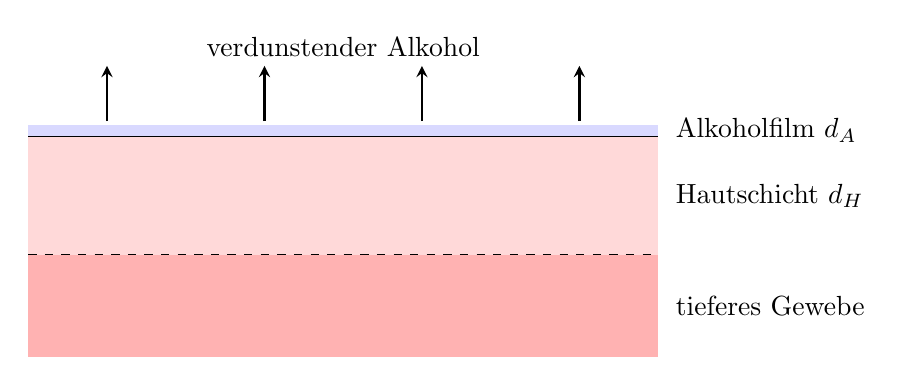
\begin{tikzpicture}[>=stealth]
 \fill[blue!15] (0,0.6) rectangle (8,0.75);
 \fill[red!15] (0,-0.9) rectangle (8,0.6);
 \fill[red!30] (0,-2.2) rectangle (8,-0.9);
 \draw (0,0.6) -- (8,0.6);
 \draw[dashed] (0,-0.9) -- (8,-0.9);
 \node[anchor=west] at (8.1,0.68) {Alkoholfilm $d_\text{A}$};
 \node[anchor=west] at (8.1,-0.15) {Hautschicht $d_\text{H}$};
 \node[anchor=west] at (8.1,-1.55) {tieferes Gewebe};
 \foreach \x in {1,3,5,7} \draw[->, thick] (\x,0.8) -- (\x,1.5);
 \node[above] at (4,1.5) {verdunstender Alkohol};
\end{tikzpicture}
\end{center}

Schätzungen: Der Alkohol (Ethanol) bildet auf der Haut einen Film von etwa $d_\text{A} = \dAO$ Dicke; die Verdampfungswärme wird hauptsächlich einer etwa $d_\text{H} = \dHO$ dicken Hautschicht entzogen, die ungefähr die Dichte $\rho_\text{H} \approx \rhHO$ und die spezifische Wärme $c_\text{H} \approx \cHO$ von Wasser hat. Mit $\rho_\text{A} = \rhEtO$ (FoTaBe S.~187) und $L_\text{v} = \LvEO$ (FoTaBe S.~191) gilt pro Fläche $A$
\begin{align}
 \rho_\text{A}A\,d_\text{A}L_\text{v} &= \rho_\text{H}A\,d_\text{H}c_\text{H}\,\Delta\vartheta
\end{align}
und damit
\begin{align}
 \Delta\vartheta &= \dTF \\
   &= \frac{\rhEt\cdot\dA\cdot\LvE}{\rhH\cdot\dH\cdot\cH} \\
   &= \dT \approx \result{\dTP{0}{1}}
\end{align}
Die Haut kann sich also um einige Grad abkühlen. Weil der Alkohol nicht schlagartig verdunstet und das Blut laufend Wärme nachliefert, ist die tatsächliche Abkühlung kleiner.
